%!TEX TS-program = xelatex
% cv-v2.7
\documentclass[hidelinks,11pt]{friggeri-cv}
\usepackage{fontawesome}
\usepackage{tikz}
\usepackage{url}
\usepackage{color}
\usepackage{graphicx}
\usetikzlibrary{decorations.markings}
\newfontfamily{\FA}[Path = fonts/]{FontAwesome}
\def\twitter{{\FA \faTwitter}}
\def\github{{\FA \faGithub}}
\def\linkedin{{\FA \faLinkedin}}
\def\envelope{{\FA \faEnvelope}}
\def\phone{{\FA \faPhone}}
\def\mobilePhone{{\FA \faMobilePhone}}
\def\book{{\FA \faBook}}
\def\flask{{\FA \faFlask}}
\def\search{{\FA \faSearch}}
\def\users{{\FA \faUsers}}
\def\pencil{{\FA \faPencil}}
\def\suitcase{{\FA \faSuitcase}}
\def\quotesymbol{{\FA \faQuote}}
\def\apple{{\FA \faApple}}
\def\windows{{\FA \faWindows}}
\def\linux{{\FA \faLinux}}
\def\circle{{\FA \faCircleFilled}}
\def\circleo{{\FA \faCircleO}}
\def\stari{{\FA \faStar}}
\def\staro{{\FA \faStarEmpty}}
\def\starhalfo{{\FA \faStarHalfO}}
\def\circlehalfo{{\FA \faCircleHalfO}}
\def\user{{\FA \faUser}}

\newcommand{\printaside}{
  \begin{aside}
  	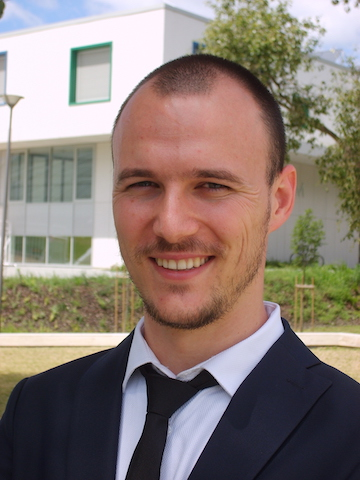
\includegraphics[width=3.3cm,keepaspectratio]{photo}
    \section{Programming}\\
    {
      	Bash {\footnotesize \textcolor{gray}{\circle\ \circle\ \circle\ \circle\ \circleo}}\\
      	C/C++/C\# {\footnotesize \textcolor{gray}{\circle\ \circle\ \circleo\ \circleo\ \circleo}}\\
        Docker {\footnotesize \textcolor{gray}{\circle\ \circle\ \circle\ \circleo\ \circleo}}\\
      	Git {\footnotesize \textcolor{gray}{\circle\ \circle\ \circle\ \circle\ \circleo}}\\
      	Java {\footnotesize \textcolor{gray}{\circle\ \circle\ \circle\ \circle\ \circleo}}\\
      	JavaScript {\footnotesize \textcolor{gray}{\circle\ \circle\ \circle\ \circleo\ \circleo}}\\
      	Python {\footnotesize \textcolor{gray}{\circle\ \circle\ \circleo\ \circleo\ \circleo}}\\
      	Spring {\footnotesize \textcolor{gray}{\circle\ \circle\ \circle\ \circleo\ \circleo}}\\
      	SQL {\footnotesize \textcolor{gray}{\circle\ \circle\ \circle\ \circle\ \circleo}}\\
     }
    \section{Operating systems}\\
      {\textcolor{gray}{\linux}\ Linux\\
      \textcolor{gray}{\apple}\ Mac OS X\\
      \textcolor{gray}{\windows}\ Windows}\\
    \section{Languages}\\
    {Working proficiency in:\\
      English {\footnotesize \textcolor{gray}{\stari\stari\stari\stari\staro}}\\
    	Hungarian {\footnotesize \textcolor{gray}{\stari\stari\stari\stari\starhalfo}}\\
    	Romanian {\footnotesize \textcolor{gray}{\stari\stari\stari\stari\starhalfo}}}\\
    \section{Contact}{
    	~\\
    	\textcolor{gray}{\mobilePhone}\ +41 76 233 2746\\
    	\href{mailto:laslaul@yahoo.com}{\textcolor{gray}{\envelope}\ laslaul@yahoo.com}\\
    	\href{https://github.com/LeonardLaszlo}{\textcolor{gray}{\github}\ LeonardLaszlo}\\
    	\href{http://www.linkedin.com/in/LeonardLaszlo}{\textcolor{gray}{\linkedin}\ Leonard László}\\
    	~\\
    	\href{https://goo.gl/maps/hmDQ8qNK5KMDU4kh9}{
    		{\boldfont Leonard László}\\
    		8134 Adliswil,\\
        Zelgstrasse 6,\\
        Switzerland\\
    	}
    }
  \end{aside}
}

\begin{document}
\header{\thinfont Leonard\ }{\boldfont László}{Senior Computer Engineer}
\printaside

\section{{\user} Recommandation \hfill {\small Péter Módos, Tech lead @ SimpledCard, \href{http://www.linkedin.com/in/LeonardLaszlo}{\textit{LinkedIn}}, July 4th, 2019)}}
Leonard worked in my team at SimpledCard as a java developer. He is very passionate about technology, he doesn't stop programming at the end of the working day, he keeps playing with new technologies also at home. As a result, he is quite up-to-date about new solutions and trends and he is happy to apply his ideas at work. He is constantly challenging the status quo, he is the driver of a lot of improvements. He likes to understand the business aspects of the work as well which would make him a productive and dedicated contributor of any software projects.

\section{{\pencil}\ Education}
\begin{entrylist}
  \entry
    {2015--2016}
    {{\normalfont Computer engineering M.Sc.}      }
    {\href{http://www.bme.hu/?language=en}{Budapest University of Technology and Economics} (\href{https://www.aut.bme.hu/en/default.aspx}{BME--AUT})}
    {Thesis title: Multi-platform multimedia application development with \textit{\href{https://nwjs.io/}{NW.js}} framework.}
  \entry
    {2011--2015}
    {{\normalfont Computer engineering B.Sc.}}
    {\href{http://www.bme.hu/?language=en}{Budapest University of Technology and Economics} (\href{http://www.mit.bme.hu/eng/}{BME--MIT})}
    {Specialised in system design. Thesis title: Cloud monitoring solutions.}
  %\smallEntry
    %{2010--2011}
    %{Studied mathematics and physics.}
    %{\href{http://www.balassiintezet.hu/en/}{Balassi Institute, Budapest}}
\end{entrylist}

\section{{\suitcase}\ Experience}
\begin{entrylist}
    \entry
    {2019--Present}
    {Senior Java Developer}
    {Move Digital AG, Zurich}
    {Currently working on the development of a quoting system.}
    \entry
    {2017--2019}
    {Software engineering}
    {SimpledCard, Budapest}
    {Accountable for reducing the errors in the payment system, pushing and implementing tech upgrades, feature design and development, plus system maintenance.}
    \entry
    {2016--2017}
    {Senior Java Developer}
    {Evosoft, Budapest}
    {Responsible for the development of a reverse proxy for an IoT cloud platform.}
    \entry
    {2014}
    {Java Developer}
    {Siwena, Budapest}
    {Authored a communication protocol implementation in Java.}
    \entry
    {2013}
    {Safety-critical software tester}
    {Testware, Budapest}
    {Responsible for safety-critical operating system testing.}
    \entry
    {Always}
    {SBC enthusiast}
    {}
    {Author of \textit{\href{https://github.com/LeonardLaszlo/nw.js-armv7-binaries}{NW.js for ARMv7}} and other \textit{\href{http://www.hardkernel.com/main/main.php}{Odroid}} and \textit{\href{https://www.raspberrypi.org}{Rpi}} single-board computer projects, such as the collection and visualisation of data points, git backbone repositories setups, database setups, file server setups and web server setups.}
\end{entrylist}

\section{{\book}\ Publications}
Multi-platform multimedia application development with NW.js framework.

Porting Popcorn Time for ARMv7 Linux devices.
{\small (Odroid Magazine, July 2015, \textit{\href{http://bit.ly/29G47yN}{http://bit.ly/29G47yN}})}

Forwarding Popcorn Time API calls through Tor network.
\end{document}
